\section{\'Etude de l'existant : ADTool}


	\label{sec:adtool}

	% Hierarchiser cette partie
	% Mettre en évidence fct qui manquent 

	ADTool permet de construire un ADTree sans difficulté. Le logiciel offre la possibilité de créer de nouveaux nœuds, d'éditer leurs labels et de leur ajouter des fils de façon simple et intuitive. Cette dernière fonctionnalité correspond à l'action « Add Child » visible sur la Figure 1. Il est aussi possible d'ajouter des frères à un nœud choisi. Le choix des opérateurs entre ces nœuds (conjonction ou disjonction)  se fait rapidement, et la mise en place de défenses est également très facile à réaliser. 
	
	\begin{figure}[h]
        \centering
        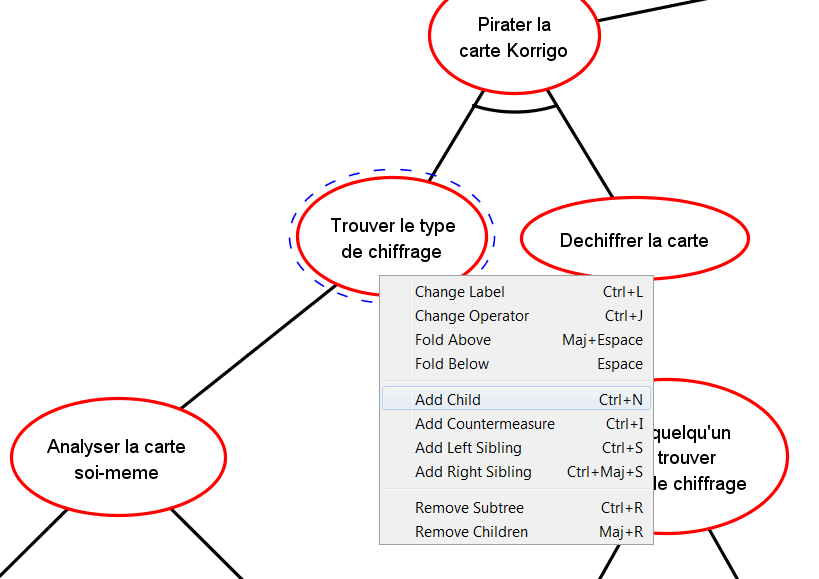
\includegraphics[width=1\textwidth]{figure/adtool_add_child.png}
        \caption{La création d'un arbre dans ADTool est simplifiée par des actions accessibles facilement.}
        \label{fig:arbre_exemple_1}
    \end{figure}
	
	Une fois l'arbre établi, il est possible d'ajouter des valuations à chaque feuille\footnote{Une feuille est un nœud n'ayant aucun fils.} de l'arbre selon un paramètre, qu'ADTool se charge ensuite de propager aux nœuds pères de façon récursive, jusqu'à la racine. ADTool dispose à l'heure actuelle de treize paramètres de base (appelés \textit{domains}), que nous allons présenter dans \textsc{table}~\ref{tab:DescriptionParam}. Nous avons repris les noms (en anglais) qui apparaissent dans le logiciel. 
					
			\begin{table*}[!h]
				\centering
				\begin{tabular}{|p{6cm}|p{5cm}|}
					\hline
					\textbf{Paramètre} & \textbf{Valeurs possibles} \\
					\hline
					Difficulty for the proponent (L,M,H) & 
						Low (bas), Medium (moyen), High (élevé) ou l'infini.\\ 
					\hline
					Difficulty for the proponent (L,M,H,E) & 
						Low (bas), Medium (moyen), High (élevé), Extreme (extrême) ou l'infini.\\ 
					\hline
					Minimal cost for the proponent (not reusable) & 
						Valeurs réelles positives, ou l'infini.\\ 
					\hline
					Minimal skill level needed for the proponent & 
						Valeurs entières positives, ou l'infini.\\ 
					\hline
					Minimal time for the proponent (in parallel) & 
						Valeurs réelles positives, ou l'infini.\\ 
					\hline
					Minimal time for the proponent (sequential) (\textit{temps minimal séquentiel}) & 
						Valeurs réelles positives, ou l'infini.\\ 
					\hline
					Overall maximal power consumption & 
						Valeurs réelles positives, ou l'infini.\\ 
					\hline
					Probability of success &
						Valeurs réelles entre 0 et 1.\\ 
					\hline
					Reachability of the proponent's goal in less than k units (in parallel) & 
						Valeurs entières de 0 à k. \\ 
					\hline
					Reachability of the proponent's goal in less than k units (sequential) & 
						Valeurs entières de 0 à k. \\ 
					\hline
					Satisfiability for the opponent & 
						Vrai ou faux. \\ 
					\hline
					Satisfiability for the proponent & 
						Vrai ou faux. \\ 
					\hline
					Satisfiability of the scenario & 
						Vrai ou faux. \\
					\hline
				\end{tabular}
				\caption{Description des paramètres}
				\label{tab:DescriptionParam}
			\end{table*}

			On voit dans le tableau ci-dessus que des termes particuliers sont utilisés pour désigner les deux parties de l'attaque : l'attaquant et le défenseur. En effet, ADTool permet de se mettre à la place de l'un ou de l'autre. Ainsi, le terme \textit{proponent} désigne l'attaquant (respectivement le défenseur) si on désire son point de vue. La racine de l'arbre représente alors l'objectif final de l'attaquant (respectivement du défenseur).L'adversaire (\textit{opponent}) est alors le défenseur (respectivement l'attaquant).
	
	\begin{figure}[h]
        \centering
        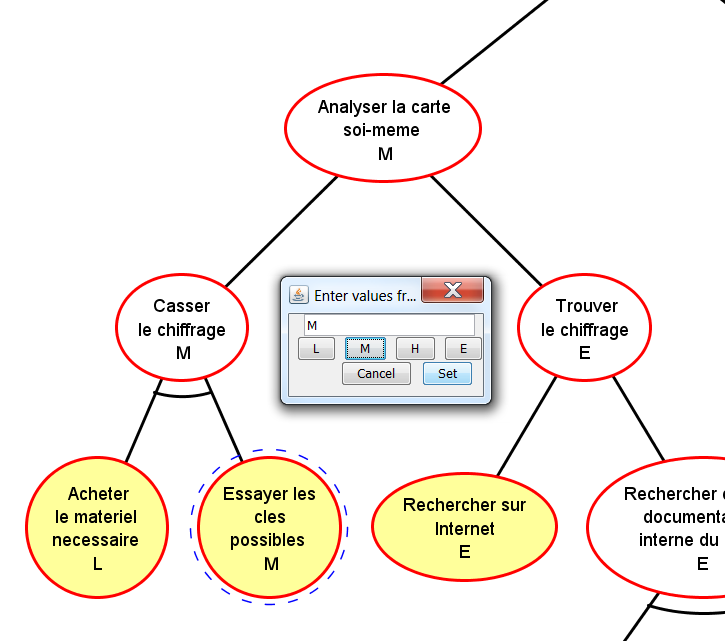
\includegraphics[width=1\textwidth]{figure/adtool_add_values.png}
        \caption{L'ajout de valuations aux feuilles est simple. Ces valuations se propagent ensuite récursivement à tous les antécédents }
        \label{fig:arbre_exemple_2}
    \end{figure}
	
	Dans l'exemple de la {\sc Figure} \ref{fig:arbre_exemple_1}, chaque noeud possède une valuation selon le paramètre de base \og difficulté de réalisation \fg{}. Comme indiqué précédemment, cette valuation peut prendre les valeurs L, M, H ou E. En éditant la difficulté de réalisation de la feuille \og essayer les clés de chiffrage possibles \fg{}  à \emph{Medium}, la valuation du nœud père \og casser le chiffrage \fg{} est recalculée pour prendre la valeur \emph{Medium} : en effet, la difficulté de ce nœud conjonctif correspond à la difficulté la plus élevée parmi ses fils. Puis, à son tour, la valuation du père de ce nœud-père est recalculée à \emph{Middle}, car, étant un nœud disjonctif, sa difficulté de réalisation correspond à la difficulté la plus faible de ses fils.
	
	L'utilisateur n'a donc pas de calcul à faire lui-même pour obtenir la valuation de la racine de son arbre, c'est-à-dire la valuation de son objectif final. Cependant, l'analyse de l'arbre ainsi construit ne va pas plus loin : ADTool ne précise pas d'où provient la valuation d'un nœud, ce qui nous amène à expliciter ci-dessous une première limitation du logiciel. Nous en avons relevé deux autres que nous décrirons juste après.\\

	 \paragraph{L'exploitation des valuations} L'utilisateur n'a aucun moyen de déterminer automatiquement le \og meilleur chemin \fg{} permettant d'atteindre la racine de l'arbre, par exemple. Il doit le déduire manuellement, en analysant la façon dont les valuations se sont propagées. Sachant qu'un arbre atteint très rapidement une taille conséquente, cette opération peut prendre un temps très important, ce qui peut être un obstacle pour l'utilisateur. C'est pourquoi nous avons décidé de pallier à ce problème en implémentant une fonctionnalité appelée \emph{Optimiseur}, que nous présenterons plus tard dans ce rapport.\\
	
	\paragraph{La visibilité des nœuds} Lorsque l'utilisateur souhaite se focaliser sur une partie de son arbre, il ne peut que masquer tous les nœuds hiérarchiquement au-dessus (ou en dessous) d'un nœud spécifique, sans distinction. Il pourrait être intéressant d'avoir la possibilité de n'afficher que les nœuds dont la valuation correspond à certains critères (difficulté acceptable, temps raisonnable, etc.), et de masquer tous les autres. Ceci permettrait à l'utilisateur de s'affranchir des nœuds et/ou des chemins qui ne l'intéressent pas, ce qui faciliterait son analyse. C'est dans cet objectif que nous allons mettre en place une fonction \emph{Filtre} décrite dans la {\sc Section} \ref{subsection:filtre}.\\

	\paragraph{L'affichage des paramètres} L'analyse de l'arbre est également restreinte par le fait que la valuation d'un nœud (et donc de l'arbre entier) ne peut se faire que selon un seul paramètre à la fois. Il n'est pas possible de prendre en compte la \og difficulté \fg{} ET le \og temps nécessaire \fg{} à la réalisation d'un nœud, par exemple. Ceci est contraignant car il est difficile de séparer ces deux notions : par exemple, le nœud \og essayer les clés de chiffrage possibles \fg{} est très facile à effectuer (il suffit de taper les clés une-à-une jusqu'à trouver la bonne), mais le temps nécessaire pour effectivement essayer chaque clé est colossal. ADTool ne permet donc pas d'obtenir une vision plus complète de l'arbre par combinaison de plusieurs paramètres. Nous souhaitons donc rendre possible l'affichage simultané de différentes valuations sur un même arbre. Nous ajouterons également la possibilité de créer des combinaisons de paramètres de base, sous la forme de \emph{paramètres de synthèse} explicités dans la section qui suit.
	 
	 
	 
